%ici je veux présenter la méthodologie et les données que j'ai utilisées 

\section{Data and Methods}


The general workflow for integrating time-series data and model is depicted in \pref{fig:workflow} and comprises the following steps:

\begin{figure*}[!t]
 \centering
 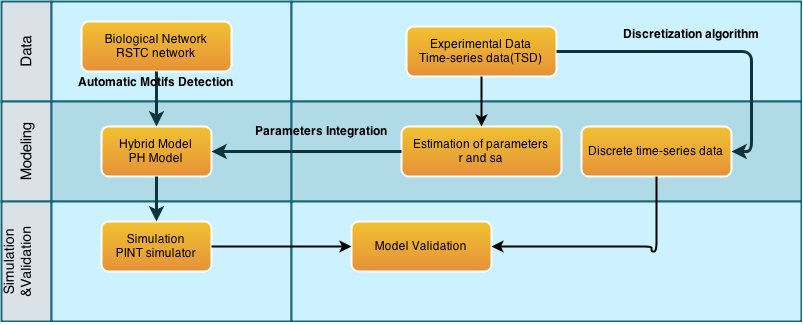
\includegraphics[width=6.5in]{images/workflow-2.png}
\caption{{\bf Workflow for integrating stochastic and temporal informations in large scale biological networks}} 
 \label{fig:workflow}
\end{figure*}

\begin{itemize}
 \item \textbf{Formalization of biological model.} Building a computational hybrid model  from biological network by automatic detection of known biological patterns.
 \item \textbf{Temporal parameters estimation.} Estimation of temporal parameters from times-series data to calibrate the model.
 \item \textbf{Integration of temporal parameters.} 
 \item \textbf{Discretization of times-series data.} Discretization of time series data to compare with discrete simulation results.
 \item \textbf{Simulation and validation.} Compare the results of simulation with the discretized times-series data.
\end{itemize}

\subsection{Data}

\subsubsection{Interaction network}
% \paragraph{The RSTC Network}
\label{ssec:RSTC}
The interactions of the biological system under study were represented in
 an RSTC network, which stands for  multi-layer receptor-signaling-transcription-cell state network, generated from the Pathway Interaction Database (PID).
In order to build this network, we selected a set of seed nodes related to the biological process studied.
The seed nodes for our case study were:  (1) \emph{E-cadherin}, which is a protein having $Ca$ binding domains and which plays an important role in cell adhesion;
(2) the $12$ significantly differentially expressed genes accross the $10$ time-points; and (3) the cell states of keratinocytes-differentiation and cell-cycle-arrest. 
The network was extracted automatically from the whole content of the NCI-PID database by using a subgraph algorithm to link the seed nodes \cite{guziolowski2012automatic}. 
In \pref{fig:network} we show the RSTC network obtained. 

\begin{definition}[RSTC Network] \label{def:RSTCDef}
A \emph{RSTC Network} $N$ is a couple $(V,E)$, where:
\begin{itemize}
\item $V =V_{T} \bigcup V_{I} $ is the finite set of \emph{nodes};
 with 
  $V_{T} = \{v_{1t},v_{2t}, \dots ,v_{n1t} \} $ the set of terminal nodes;
  $V_{I} = \{v_{1i},v_{2i}, \dots ,v_{n2i} \} $ the set of transient nodes.
\item $E = \{e_{1},e_{2}, \dots, e_{m} \}$ is the set of edges. $ E \subseteq (V_{T} \times V_{T}) \bigcup (V_{T} \times V_{I}) 
\bigcup (V_{I} \times V_{T})$
\end{itemize}
\end{definition}

In this definition, terminal nodes can be genes, proteins, complexes, cellular state, biological processes and positive condition. 
On the other side, transient nodes can be transcriptions, translocations, modifications and compounds. Edges are of different types.
We have activation (agent), inhibition, output, input and famillyMemberOf.

\begin{figure*}[!t]
 \centering
 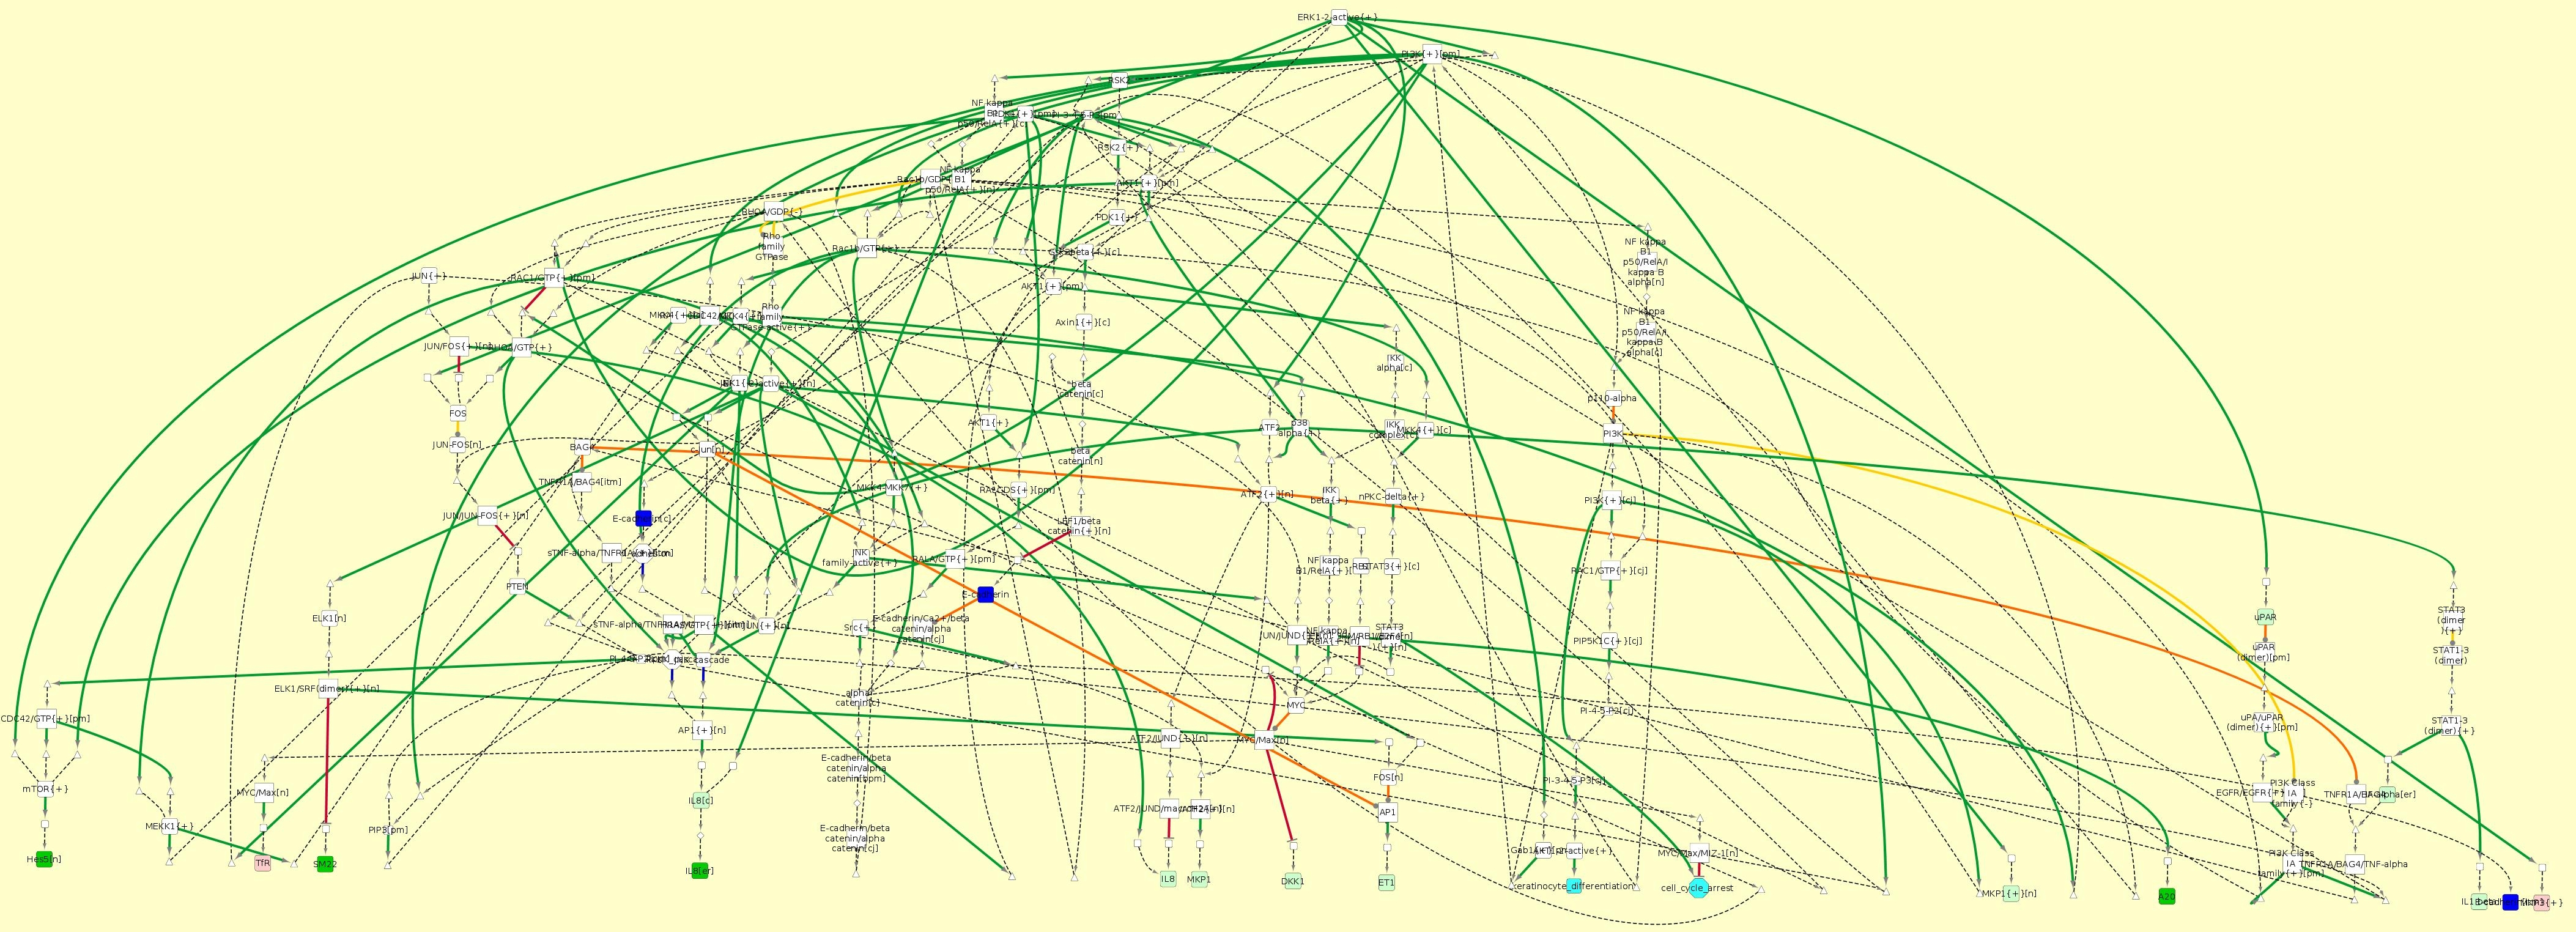
\includegraphics[width=6.5in]{images/net.jpg}
\caption{{\bf RSTC network. It is the interaction graph that describe the biological case study. It is composed of $293$ nodes and $375$ edges (interactions).
The set of nodes are composed of terminal nodes(proteins, complexes, genes, cellular state, biological processes and positive conditions) and of transient
nodes (transcriptions, compound, translocations, modifications and compounds). The set of edges are composed of interactions of type activation (agent), inhibition, output, 
input and famillyMemberOf}} 
 \label{fig:network}
\end{figure*}

%description des données
\subsubsection{Time-series microarray data description}
\label{SECTSD}
To illustrate our approach, we used the time-series microarray data from Calcium stimulated keratinocyte cells 
 measured at $10$ time-points. A $200$ transcripts were selected for their dynamic patterns,
that is, their fold expression with respect to the non-stimulated cell was significant in at least one time point. 
We included in our model a set of $12$ of the $200$ selected (see \pref{fig:tsd}), because we were able to retrieve the regulatory mechanisms upstream
these $12$ genes from public repositories of biochemical reactions.
The full dataset (data not shown) was produced by the German Cancer Research Center (DKFZ) and it's currently in the process
of getting published.  

\begin{figure}[!t]
\centering
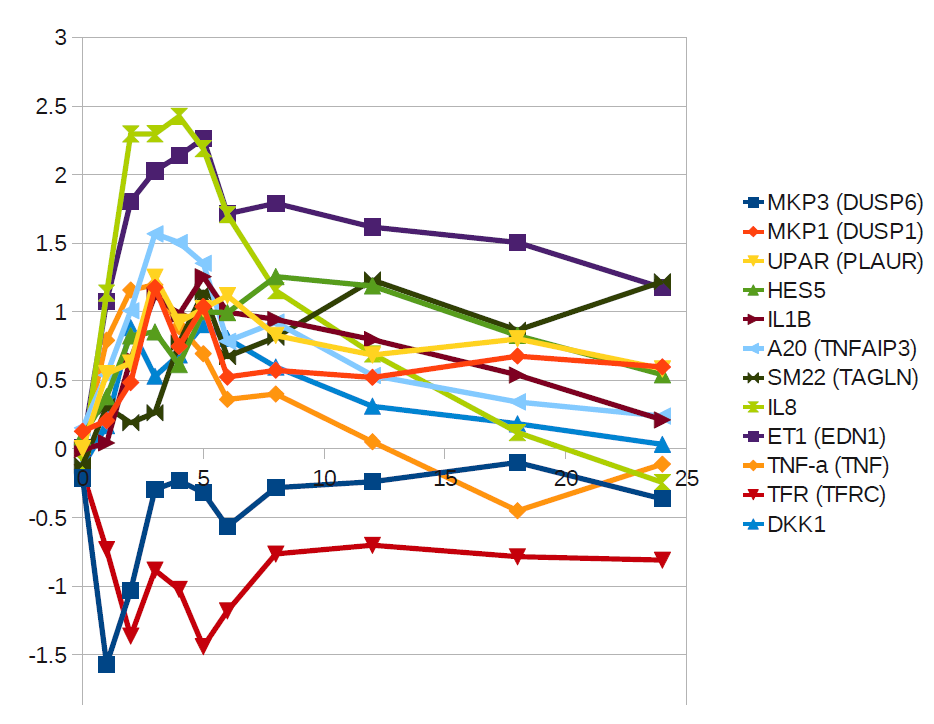
\includegraphics[width=2.5in]{images/12genes.png}
\caption{\bf Plot of $12$ selected genes}
\label{fig:tsd}
\end{figure}


\subsection{The Process  Hitting Framework}
\label{ssec:PH}

%We present here the Process Hitting framework \cite{PMR10-TCSB} which will enable us to model 
%biological network.

%\vspace{3mm}

Process Hitting (PH) gathers a finite number of concurrent processes grouped into a finite set of sorts.
A sort stands for a component of a biological system while a process, which belongs to a unique sort, stands
for one of its expression levels. At any time, exactly one process of each sort is present. A state of the 
PH corresponds to such a set of processes. We denote here a process by $a_i$ where $a$ 
is the sort and $i$ is the process identifier within the sort $a$.
The concurrent interactions between processes are defined by a set of \emph{actions}.
Actions describe the replacement of a process by another of the same sort conditioned by the presence 
of at most one other process in the current state. An action is denoted by $\PHfrappe{a_i}{b_j}{b_k}$, 
which is read as ``$a_i$ \emph{hits} $b_j$ to make it bounce to $b_k$'', where $a_i,b_j,b_k$ are 
processes of sorts $a$ and $b$, called respectively \emph{hitter}, \emph{target} and \emph{bounce} of 
the action.

\begin{definition}[Process Hitting] \label{def:PH}
A \emph{Process Hitting} is a triple $(\PHs,\PHl,\PHa)$, where:
\begin{itemize}
\item $\PHs = \{a,b,\dots\}$ is the finite set of \emph{sorts};
\item $\PHl = \prod_{a\in\PHs} \PHl_a$ is the set of states with $\PHl_a = \{a_0,\dots,a_{l_a}\}$
the finite set of \emph{processes} of sort $a\in\Sigma$ and $l_a$ a positive integer, with $a\neq b\Rightarrow \PHl_a \cap \PHl_b = \emptyset$;
\item $\PHa = \{ \PHfrappe{a_i}{b_j}{b_k} \in \PHl_a \times \PHl_b \times \PHl_b \mid (a,b) \in \PHs^2
  \wedge b_j\neq b_k \wedge a=b\Rightarrow a_i=b_j\}$ is the finite set of \emph{actions}.
\end{itemize}
\end{definition}

\noindent
Given a state $s\in \PHl$, the process of sort $a\in\PHs$ present in $s$ is denoted by $\PHget{s}{a}$.
An action $h=\PHfrappe{a_i}{b_j}{b_k} \in \PHa$ is \emph{playable} in $s \in L$ if and only if $\PHget{s}{a}=a_i$ and $\PHget{s}{b} = b_j$.
In such a case, $(s\play h)$ stands for the state resulting from the play of the action $h$ in $s$, with
$\PHget{(s\play h)}{b} = b_k$ and $\forall c \in \PHs, c \neq b, \PHget{(s\play h)}{c} = \PHget{s}{c}$.

\subsubsection{Modeling cooperation}

As described in \cite{PMR10-TCSB}, the cooperation between processes to make another process bounce can be
expressed in PH by building a \emph{cooperative sort}.
\pref{fig:runningPH} shows an example of a cooperative sort $ab$ between sorts $a$ and $b$,
defined with 4 processes (one for each sub-state of the presence of processes $a_1$ and $b_1$).
For the sake of clarity, processes of $ab$ are indexed using the sub-state they represent.
Hence, $ab_{01}$ represents the sub-state $\PHstate{a_0,b_1}$, and so on.
Each process of sort $a$ and $b$ hit $ab$, which makes it bounce to the process reflecting the status of the sorts $a$
and $b$ (e.g., $\PHfrappe{a_1}{ab_{00}}{ab_{10}}$ and $\PHfrappe{a_1}{ab_{01}}{ab_{11}}$).
Then, to represent the cooperation between processes $a_1$ and $b_1$,
the process $ab_{11}$ hits $c_1$ to make it bounce to $c_2$ instead of
independent hits from $a_1$ and $b_1$.
The same cooperative sort is used to make $a_0$ and $b_0$ cooperate to hit $c_1$ and make it bounce to $c_0$.
\subsubsection{Modeling synchronization}
%introdure la synchronization
Unlike cooperation sort which allow us to model the fact that two components cooperate to hit another component, we introduce
the notion of synchronization sort, which will implement another type of cooperation. If we refer to our example
\pref{fig:runningPH}, and asume that $ab$ is our \emph{synchronization sort} between sorts $a$ and $b$, defined with also 
4 processes. Then, component $c$ will be activated ($c_1$ bounce to $c_2$) if each one of $a$ and $b$ are also activated. So each 
one of this processes $ab_1$, $ab_2$, $ab_3$ can activate $c_1$. But to be desactived, we need both $a$ and $b$ to be desactived.
We will see later why it is important to introduce this new rule for the cooperation between componnets in our real case study.

Remember that PH was designed in order to take very large system analysis into account. Indeed, algorithm were developped on such a
process??? system so that it prevent for building the whole state graph which would be intractable when there are more than $10$ or 
$20$ components.

\begin{example}
\pref{fig:runningPH} represents a PH $(\PHs,\PHl,\PHa)$ with $\PHs = \{a,b,c,ab\}$, and:
\begin{align*}
\PHl_a &= \{a_0,a_1\},\\
\PHl_b &= \{b_0, b_1\},\\
\PHl_{ab} &= \{ab_{00}, ab_{01}, ab_{10}, ab_{11}\},&\\
\PHl_c &= \{c_0, c_1, c_2\}.
\end{align*}
This example models a Biological Regulatory Network (BRN) where the component $c$ has three qualitative levels, components $a$ and $b$ are Boolean and $ab$ is a cooperative sort.
In this BRN, $ab$ inhibits $c$ at level $2$ through the cooperative sort $ab$ (e.g. $\PHfrappe{ab_{00}}{c_2}{c_1}$, $\PHfrappe{ab_{00}}{c_1}{c_0}$) while $a$ and $b$ activate $c$  
through the cooperative sort $ab$ (e.g. $\PHfrappe{ab_{11}}{c_0}{c_1}$ $\PHfrappe{ab_{11}}{c_1}{c_2}$ ). Indeed, the reachability of $c_2$ and $c_0$ 
is conditioned by a cooperation of $a$ and $b$, as explained above.

\begin{figure}[!t]
%\centering
\begin{minipage}{0.3\linewidth}
\centering
\scalebox{0.7}{
\begin{tikzpicture}[grn]
\path[use as bounding box] (-0.2,-0.7) rectangle (3.5,0.7);
\node[inner sep=0] (a) at (1,2) {a};
\node[inner sep=0] (b) at (1,0) {b};
\node[inner sep=0] (c) at (3,1) {c};
\path[->]
  (b) edge node[elabel, above=-3pt] {$+$} (c)
  %(c) edge node[elabel, above=-5pt] {$1+$} (a)
  (a) edge node[elabel, above=-3pt] {$+$} (c);
\end{tikzpicture}
}
\end{minipage}
\begin{minipage}{0.7\linewidth}
\centering
\scalebox{0.7}{
\begin{tikzpicture}
\path[use as bounding box] (-2,-5.2) rectangle (7,0.7);

\TSort{(0,0)}{a}{2}{t}
\TSort{(0,-3.8)}{b}{2}{b}
\TSort{(4.5,-3)}{c}{3}{r}

\TSetTick{ab}{0}{00}
\TSetTick{ab}{1}{01}
\TSetTick{ab}{2}{10}
\TSetTick{ab}{3}{11}
\TSort{(-0.5,-2)}{ab}{4}{b}


\THit{a_1}{bend right}{ab_0}{.north}{ab_2}
\THit{a_1}{bend right}{ab_1}{.north}{ab_3}
\THit{a_0}{}{ab_2}{.north west}{ab_0}
\THit{a_0}{}{ab_3}{.north west}{ab_1}

\THit{b_0}{}{ab_1}{.south}{ab_0}
\THit{b_0}{}{ab_3}{.south}{ab_2}
\THit{b_1}{}{ab_0}{.south}{ab_1}
\THit{b_1}{}{ab_2}{.south}{ab_3}

\path[bounce, bend right=25]
\TBounce{ab_2}{}{ab_0}{.north east}
\TBounce{ab_3}{}{ab_1}{.north east}
;
\path[bounce, bend left=80, distance=30]
\TBounce{ab_0}{}{ab_2}{.north}
\TBounce{ab_1}{}{ab_3}{.north}
;
\path[bounce, bend right]
\TBounce{ab_0}{}{ab_1}{.west}
\TBounce{ab_2}{}{ab_3}{.west}
;
\path[bounce, bend left]
\TBounce{ab_3}{}{ab_2}{.east}
\TBounce{ab_1}{}{ab_0}{.east}
;

\THit{ab_3}{thick}{c_1}{.north west}{c_2}
\THit{ab_0}{thick,bend right=130, in=305, distance=140}{c_1}{.south east}{c_0}
\path[bounce, bend left=40]
\TBounce{c_1}{thick}{c_2}{.south west}
\TBounce{c_1}{thick}{c_0}{.north east}
;

\THit{ab_3}{thick}{c_0}{.north west}{c_1}
\THit{ab_0}{thick,bend right=130, in=305, distance=140}{c_2}{.south east}{c_1}
\path[bounce, bend left=40]
\TBounce{c_0}{thick}{c_1}{.south west}
\TBounce{c_2}{thick}{c_1}{.north east}
;


\end{tikzpicture}
}
\end{minipage}

\caption{\label{fig:modelingBRN}
(left)~Biological pattern example.
Nodes are components and edges are interactions
For instance, components $a$ and $b$ cooperate to activate $c$.
(right)~equivalent PH model. \label{fig:runningPH}
A PH example with four sorts: three components ($a$, $b$ and $c$) and a cooperative sort ($ab$).
Actions targeting processes of $c$ are in thick lines.
}
\end{figure}

\end{example}




%la traduction automatique des patterns d'un réseau
\subsection{Model construction(From RSTC to PH)}
%In this part we will describe how to go from rstc to ph model
In this work, we aim to model a biological  system according to his dynamic. For that, we choose to build a PH model from the biological model reprensented as  an RSTC network.

%why we made this choice?
In the following we present our automatic approach to generate a PH model from an RSTC network.


\subsubsection{Modeling the RSTC network as a PH model}

%In this section, we present the modelisation of biological network express with the biochemical reactions in PID. In the following, we will
%present how to transform biological pattern to the PH model. After that, we propose a way of estimating temporal and stochastic
%parameters for the process hitting model. This section will end by the generation of the PH code generation for the simulation.

%\paragraph{Modeling biological patterns to PH model}

%Here is the first and the most important part of this work. 
In order to model the RSTC network as a PH model we selected known biological regulatory patterns (atomic set of biological components and their interacting roles), represented 
as biochemical reactions in the RSTC network, and proposed their PH representation. 

%les ajouts pour les patterns 
We build an algorithm that will automatically browse the graph node by node and detect all patterns in the graph. More precisely, for each node(output node of the pattern) we will call a recursive procedure,
that will allow us to detect a minimal set of node(input node of the pattern) that has an direct influence on that node. This set of node plus the output node and the way there are linked are a pattern for us. 
The type of a pattern is determine by the type of the output node, the type of regulations come on that node and the type of input nodes of the pattern. So the algorithm that detect patterns return the pattern 
and its type to another procedure which one will traduce the pattern into the process hitting formalism. This transformation will take care of different case(cooperation, synchronization, simple activation, simple inhibition,...)



%nous avons des noeuds qui sont des composants du réseau, pour notre alogorithme(récursif) ils seront considérés comme noeuds initiaux et terminaux.
%nous avons des noeuds transitoires qui relient deux arrêtes entre elles afin d'indicquer la nature de l'interaction entre deux composants terminaux
%nous avons enfin les arrêtes qui relient les noeuds terminaux aux noeuds transitoires


%%%%algorithm of patterns detection in all the network

\begin{figure}[!t]
\begin{algorithmic}[1]
%\Procedure{patternDetection}{$Net,n$}\Comment{Given a node n, detect a set of minimal nodes that has a direct regulatory effect on n}
\REQUIRE $Net$
\ENSURE return all the patterns associated to the given network $Net$
\FORALL{ Node $n$ in $Net$ } 
\STATE $Pat$ = detectPattern($Net$, $n$)
\STATE patternInPHModel($out$,$Pat$)

\ENDFOR
%\STATE \textbf{return} $b$%\Comment{The gcd is b}
\end{algorithmic}
\caption{\bf Pattern detection in an RSTC Network}
\label{patternDetection}
\end{figure}


%%%%%algorithm for detect the pattern of a given node

\begin{figure}[!t]
\begin{algorithmic}[1]
%\Procedure{patternInPHModel}{$out,Pat$}\Comment{Write on the flux out the PH Model of a given pattern (Pat)}
\REQUIRE $Net$, $n$
\ENSURE Detect a pattern associated to a given node (n in this case)
%\WHILE{$r\not=0$}  %\Comment{We have the answer if r is 0}
\STATE 
\STATE 
\SWITCH {$n$}
 \CASE{TerminalNode} %\COMMENT{We compact many sub case of all terminal nodes}
   \STATE added node to the pattern
   \STATE numberPredecessor= $n$.getNumberOfPredecessor() \COMMENT{To get the number of predecessor of node $n$}
   \SWITCH{numberPredecessor}
   
   \CASE{1}
    \FORALL {in comming edge (n-m)}
    \STATE get the node $m$
    \SWITCH {$m$}
    \CASE {TerminalNode}
      \STATE added node to the pattern $Pat$
    \ENDCASE
    
    \CASE {TransientNode}
      \STATE detectPattern($Net$,$m$);
    \ENDCASE
    
    \ENDSWITCH
   \ENDFOR
      \STATE Set the code of pattern Pat
      \STATE return $Pat$
   \ENDCASE
   
     % \CASE {2}
  % \ENDCASE
  % \DEFAULT
  %  \STATE \RETURN ERROR CODE \COMMENT{We can't treat this case}
  % \ENDDEFAULT
   \ENDSWITCH
\ENDCASE
   
   \CASE{TransientNode} %\COMMENT{We compact many sub case of all terminal nodes}
   %\STATE added node to the pattern
   \STATE numberPredecessor= $n$.getNumberOfPredecessor() \COMMENT{To get the number of predecessor of node $n$}
   \SWITCH{numberPredecessor}
   
   \CASE{1}
    \FORALL {in comming edge (n-m)}
    \STATE get the node $m$
    \SWITCH {$m$}
    \CASE {TerminalNode}
      \STATE added node to the pattern $Pat$
    \ENDCASE
    
    \CASE {TransientNode}
      \STATE detectPattern($Net$,$m$);
    \ENDCASE
    
    \ENDSWITCH
   \ENDFOR
      \STATE Set the code of pattern Pat
      \STATE return $Pat$
   \ENDCASE
   
  % \CASE {2}
  % \ENDCASE
  % \DEFAULT
  %  \STATE \RETURN ERROR CODE \COMMENT{We can't treat this case}
  % \ENDDEFAULT
   \ENDSWITCH
\ENDCASE
%\CASELINE {2}
%  \STATE Good-bye
%\DEFAULT
%  \STATE Again ?
%\ENDDEFAULT
\ENDSWITCH
%\ENDWHILE\label{euclidendwhile}
\end{algorithmic}
\caption{\bf Detection of Pattern associated to the node n} \label{PatternDetectionNode}
\end{figure}



%%%%%algorithm for write the pattern in PH model

\begin{figure}[!t]
\begin{algorithmic}[1]
%\Procedure{patternInPHModel}{$out,Pat$}\Comment{Write on the flux out the PH Model of a given pattern (Pat)}
\REQUIRE $out$, $Pat$ \COMMENT{ Pat is The pattern to be translate into the PH Model, out is the output file}
\ENSURE The correspondant PH Model of the given pattern Pat will write into the file $out$
%\WHILE{$r\not=0$}  %\Comment{We have the answer if r is 0}
\STATE $nocp$ = $Pat$.getNumberOfComponents() \COMMENT{Number of the components of the pattern $Pat$}
\STATE 
\SWITCH {$nocp$}
 \CASE {2}
  \SWITCH {$type$}
 \CASE {A}
   \STATE out.write("activation")
   \STATE out.write("")
        
\ENDCASE
\CASELINE {I}
  \STATE out.write("inhibition")
  \STATE 
\DEFAULT
 \STATE out.write("unknow pattern")
 \ENDDEFAULT
\ENDSWITCH
   
   
\ENDCASE

\CASE {3}
  \SWITCH {$type$}
 \CASE {C}
   \STATE out.write("cooperation")
        
\ENDCASE
\CASELINE {S}
  \STATE out.write("synchronization")
\DEFAULT
 \STATE out.write("unknow pattern")
 \ENDDEFAULT
\ENDSWITCH
   
   
\ENDCASE
%\CASELINE {2}
%  \STATE Good-bye
%\DEFAULT
%  \STATE Again ?
%\ENDDEFAULT
\ENDSWITCH
%\ENDWHILE\label{euclidendwhile}
\end{algorithmic}
\caption{\bf Pattern in PH Model} \label{PHModel}
\end{figure}


% les détails sur comment les patterns sont choisis 
For example a molecule $a$ that cooperates with a molecule $b$ to activate a molecule $c$ \pref{fig:runningPH} (top), is a regulatory pattern because it is a protein-complex biochemical reaction that appears recurrent times.  
We model this pattern by four sorts \pref{fig:runningPH} (bottom) $a$, $b$, $c$ and $ab$. Sorts $a$, $b$ and $c$
represent components $a$, $b$ and $c$. We introduce the cooperative sort $ab$ to characterize constraints on components $a$ and $b$.
In our RSTC network, we found $11$(to be precise...) regulatory patterns (see Appendix \ref{table_patterns}). 

\begin{table}[!t]
\renewcommand{\arraystretch}{1.3}
\caption{Examples of patterns}
\label{table_patterns}
\centering
\begin{tabular}{c||c}
\hline
\bfseries Biological Patterns

&

\bfseries PH Transformations\\ 
\hline\hline
\begin{tikzpicture}
\node[scale=0.5] (sa1) at (0,0){\begin{tikzpicture}[auto]
\path[use as bounding box] (-0.7,-0.3) rectangle (2.5,2);

\node[qgre] (a) at (0,1) {a};
\node[mod] (i) at (1,1) {i};
\node[qgre] (b) at (2,1) {b};
\node[es] (d) at (1,2) {Simple activation};

\path
 (a) edge[act] (i)
 (i) edge[st]  (b);
\end{tikzpicture}};
\end{tikzpicture}

&


\begin{tikzpicture}
%\exphpatact
\node[scale=0.5] (sa) at (0,0) {\begin{tikzpicture}
\path[use as bounding box] (-0.5,-0.5) rectangle (2.5,2.5);

\TSort{(0,0.5)}{a}{2}{l}
\TSort{(2,0.5)}{b}{2}{l}
%\TSort{(6,1)}{z}{3}{r}

\THit{a_1}{}{b_0}{.west}{b_1}
\THit{a_0}{}{b_1}{.west}{b_0}
%\THit{a_0}{out=250,in=200,selfhit}{a_0}{.west}{a_1}

\path[bounce,bend left]
\TBounce{b_0}{}{b_1}{.south}
\TBounce{b_1}{bend right}{b_0}{.north}
%\TBounce{a_0}{}{a_1}{.south}
;
\end{tikzpicture}};
\end{tikzpicture}\\ 
\hline\hline

\begin{tikzpicture}
\node[scale=0.5] (si1) at (0,0){\begin{tikzpicture}[auto]
\path[use as bounding box] (-0.7,-0.3) rectangle (2.5,2);

\node[qgre] (a) at (0,1) {a};
\node[mod] (i) at (1,1) {i};
\node[qgre] (b) at (2,1) {b};
\node[es] (d) at (1,2) {Simple inhibition};
\path
 (a) edge[inh] (i)
 (i) edge[st]  (b);
 \end{tikzpicture}};
\end{tikzpicture}

&

\begin{tikzpicture}
%\exphpatact
\node[scale=0.5] (sa) at (0,0) {\begin{tikzpicture}
\path[use as bounding box] (-0.5,-0.5) rectangle (2.5,2.5);

\TSort{(0,0.5)}{a}{2}{l}
\TSort{(2,0.5)}{b}{2}{l}
%\TSort{(6,1)}{z}{3}{r}

\THit{a_1}{}{b_1}{.west}{b_0}
\THit{a_0}{}{b_0}{.west}{b_1}
%\THit{a_0}{out=250,in=200,selfhit}{a_0}{.west}{a_1}

\path[bounce,bend left]
\TBounce{b_1}{bend right}{b_0}{.north}
\TBounce{b_0}{}{b_1}{.south}
%\TBounce{a_0}{}{a_1}{.south}
;
\end{tikzpicture}};
\end{tikzpicture}\\ 
\hline\hline

\begin{tikzpicture}
\node[scale=0.5] (sai1) at (0,0){\begin{tikzpicture}[auto]
\path[use as bounding box] (-0.7,-0.3) rectangle (2.5,3);
\node[qgre] (a) at (0,2) {a};
\node[mod] (i) at (1,1) {i};
\node[qgre] (b) at (0,0) {b};
\node[qgre] (c) at (2,1) {c};
\node[es] (d) at (1,3) {activation or inhibition};

\path
 (a) edge[act] (i)
 (b) edge[inh] (i)
 (i) edge[st]  (c);
\end{tikzpicture}};
\end{tikzpicture}


&

\begin{tikzpicture}
%\exphpatact
\node[scale=0.5] (sai) at (0,0) {\begin{tikzpicture}
\path[use as bounding box] (-0.5,-0.5) rectangle (2.5,5.5);

\TSort{(0,0)}{a}{2}{l}
\TSort{(0,3)}{b}{2}{l}
\TSort{(2,1)}{c}{2}{r}

\THit{a_1}{}{c_0}{.west}{c_1}
\THit{a_0}{}{c_1}{.west}{c_0}
\THit{b_1}{}{c_1}{.west}{c_0}
\THit{b_0}{}{c_0}{.west}{c_1}

%\THit{a_0}{out=250,in=200,selfhit}{a_0}{.west}{a_1}

\path[bounce,bend left]
\TBounce{c_1}{bend right}{c_0}{.north}
\TBounce{c_0}{}{c_1}{.south}
%\TBounce{a_0}{}{a_1}{.south}
;
\end{tikzpicture}};
\end{tikzpicture} \\
\hline
\end{tabular}
\end{table}




%\subsubsection{Integrating parameters from  time-series gene expression data}

% the goal of this section (expliquer comment et pourquoi nous allons partir des séries temporelles pour estimer les rates des actions
%This section will present how we introduce temporal feature into a formal model. The temporal informations come from TSD and we want to emphases the notion of chronometric
%or delay. 





\subsubsection{Estimating the parameters for the PH-simulation from time-series gene expression data}

%peut etre penser à faire un schéma

The simulation of the execution of the PH actions is done stochastically.  Therefore, we need to relate each action with temporal 
and stochastic parameters, introduced into the PH framework to achieve dynamic refinement \cite{PMR10-TCSB}. 
This is an important aspect of the modeling when taking into account the temporal and stochastic dimensions of 
biological reactions by performing simulations. 
On the one hand, we consider the probability of a reaction to occur, and on the other hand, we 
consider stochastic parameters in the aim at observing an expected behavior. 
In the PH framework, to play an action we need two essential parameters: the rate $r$ or the temporal parameter because $t=r^{-1}$ if we assume that $t$ is the average time of playing an action
and the stochasticity absorption $sa$. These two parameters will be estimated according to the expression profile of time-series data of the experiment
described in Section \ref{SECTSD}. 


%To avoid over fitting in the estimation of these parameters, we propose that each component of the PH, representing a measured gene in the network,  will take the estimated values of the parameters of its respective cluster in the experimental data.



%\begin{enumerate}
% \item The first step is to cluster the data set. The goal of the clustering process is to partition genes into groups such that the 
% profiles contained in the same group (cluster) are similar to each other and as different as possible from the profiles assigned to the other
% clusters. The particularity here is to choose the best clustering criteria.
% \item For each cluster obtained in the previous step, estimate the value of $r$ and $sa$ associated to the cluster.
% \item For each component of the PH model associated to the measured gene, determine its cluster, and assign it $r$ and $sa$, the previously  estimated  parameters.
%\end{enumerate}

%In our time-series data the components of the PH which need to be associated specific parameters (step 3) are the $12$ genes present in our RSTC network.

\begin{figure}[!t]
\centering

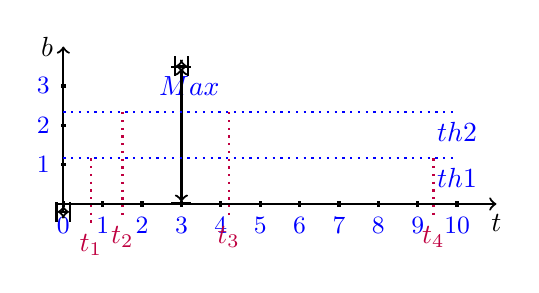
\begin{tikzpicture}[scale = 0.5]
       
    
	      \draw[thick, ->] (-.2,0)--(11,0) node[below]{$t$};
	      \foreach \t in {0,1,2,3,4,...,10}
	      \draw[very thick] (\t,2pt)--(\t,-2pt) node[below,blue]{\small\t};

	      \draw[thick, ->] (0,-.2)--(0,4) node[left]{$b$};
	      \foreach \y in {1,2,3}
	      \draw[very thick] (2pt,\y)--(-2pt,\y) node[left,blue]{\small\y};
      
	      \draw[thick] plot[mark=ball,mark size=1pt] file {illustration.txt};
    
	      %\pause
	      \draw[thick,|<->|] (2.8,3.5) -- (3.2,3.5) node[below,blue]{$Max$};
	      \draw[thick,|<->|] (-.2,-.2) -- (.2,-.2) node[below,blue]{};
	      %\pause
	      \draw[thick,|<->|] (3,0) -- (3,3.5);
	      %\pause
	      \draw[thick,dotted,blue] (0,1.16) -- (10,1.16) node[below]{$th1$}; 
	      \draw[thick,dotted,blue] (0,2.33) -- (10,2.33) node[below]{$th2$}; 
	      %\pause
	      \draw[thick,dotted,purple] (0.7,1.16) -- (0.7,-.5) node[below]{$t_{1}$};
	      %\pause
	      \draw[thick,dotted,purple] (1.5,2.33) -- (1.5,-.3) node[below]{$t_{2}$};
	      %\pause
	      \draw[thick,dotted,purple] (4.2,2.33) -- (4.2,-.3) node[below]{$t_{3}$};
	      %\pause
	      \draw[thick,dotted,purple] (9.4,1.16) -- (9.4,-.3) node[below]{$t_{4}$};

           \end{tikzpicture}
	    

\caption{Illustration of estimation of temporal parameters:$r_{i}=\frac{1}{t_{i}-t_{i-1}}$}
\label{fig:estimationParameter}
\end{figure}

\subsubsection{From data to action parameters}

%l'Introduction des données temporelles n'était pas automatique, de plus on ne savait pas le faire des données des séries temporelles.
Before this work, it were not possible to infer temporal parameters from TSD and integrate them automatically into a model build in to the process hitting formalism.
It's now possible. For components that we have measured, we know how to estimate and integrate parameters. For others that we don't have measured, we can give default parameters.



%discretisation des données
\subsubsection{Discretization of times-series data}

Because PH simulation is discrete we need to discretize continuous experimental data, so we can compare our simulation outputs.
The goal of this method was to better determine, according to the gene expression level, when  a given molecule is activated or inhibited.
To do this, we introduced the new analog concept of Significant Increase or Decrease to characterize the fact that a level of a molecule 
increases or decreases when crossing a threshold of significance; we limited the possible expression levels for a molecule to
$\{0, 1, 2\}$. We made this choice because when we look our time-series data (see \pref{fig:tsd}), we can clearly observe a high level of
activity between $0h$ and $5h$ on one hand, and a slow level of activities between $5h$ and $10h$ on the other hand. In our discretization
method, our goal is to capture this two times of activities. For achieve this goal, we propose the following discretization method.
For each time-series, we introduce two thresholds \emph{th1} and \emph{th2} as in \pref{fig:estimationParameter}. The value of this two
thresholds is compute has follow $\emph{th1}=\frac{1}{3}(MaxLevel-MinLevel)$ and $\emph{th2}=\frac{2}{3}(MaxLevel-MinLevel)$. Therefore, all
the expression level of a time-series between $[0-th1]$ will have level $0$, all those between $[th1-th2]$ will have level $1$ and the last group will
have level $2$. By this way, we can automatically determine the differents level of expression of all our time-series data. 
%illustration des résultats de la méthode de discrétisation
To illustrate the result of our discretization algorithm, we plot in \pref{fig:illustrationDiscretisation} the expression 
of $9$ seleted genes from the times-series data with their respective discrete plots. 
%On the discrete plot, one can clearly differentiate when a molecule is active or not, which is of extreme importance 
%swhen modeling these steps in the PH framework if we would like to have coherent simulation results.

\begin{figure*}[!t]
 \centering
 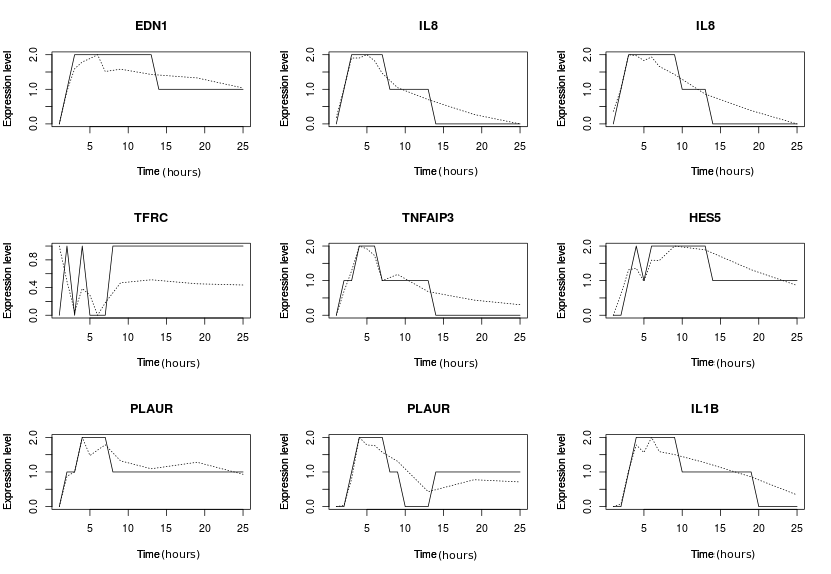
\includegraphics[width=6.5in,height=3.5in]{images/ResultDiscretization.png}
 % IllustrationDiscretisation.png: 831x574 pixel, 72dpi, 29.32x20.25 cm, bb=0 0 831 574
 \caption{Illustration of discretization of experimental data. Continous lines are descrite data, dashed lines are continuous data}
 \label{fig:illustrationDiscretisation}
\end{figure*}

  


\subsection{Simulation: Initials conditions}
%we give the initial condition for the simulation
To better understand the results of simulation, we need to give initial conditions for the components of our network. Because the components of the network are group into 
layers, the initial conditions will be the same in the different layers. In the following we will present the initial conditions that we have chosen for the different 
components.

\begin{itemize}
 \item \textbf{Receptor layer: E-cadherin.} We choose the  pulse signal for the input node E-cadherin, that will be active for a duration of average $x$ units times. We made this 
 choise to take into account the average time of calcium stimuli effect.
 \item \textbf{Signaling layer: signaling proteins.} At this layer, the components will be activated and inhibited according to the same rate and the same stochasticity absorption factor.
 The values of this parameters where selected by considering the time of signal transduction from the entry node(E-cadherin) to the output node (genes).
 \item \textbf{Transcription layer: Transcription factors.} At this stage, the signal will come from signaling proteins for activation. But for the inhibition, in addition 
 of the signal come from signaling proteins, we introduce an auto-inhibition which will represented a degradation of the transcription factor.
 \item \textbf{Cell-state: Gene and cellular  process.} The genes will be activited or inhibited according to the estimated values from time-series data.
\end{itemize}

We summarise the initial conditions of our simulation in \pref{fig:initialCondition} were we can clearly see the initial values choose at each layer for our model.

\begin{figure}[!t]
 \centering
 \scalebox{0.45}{
  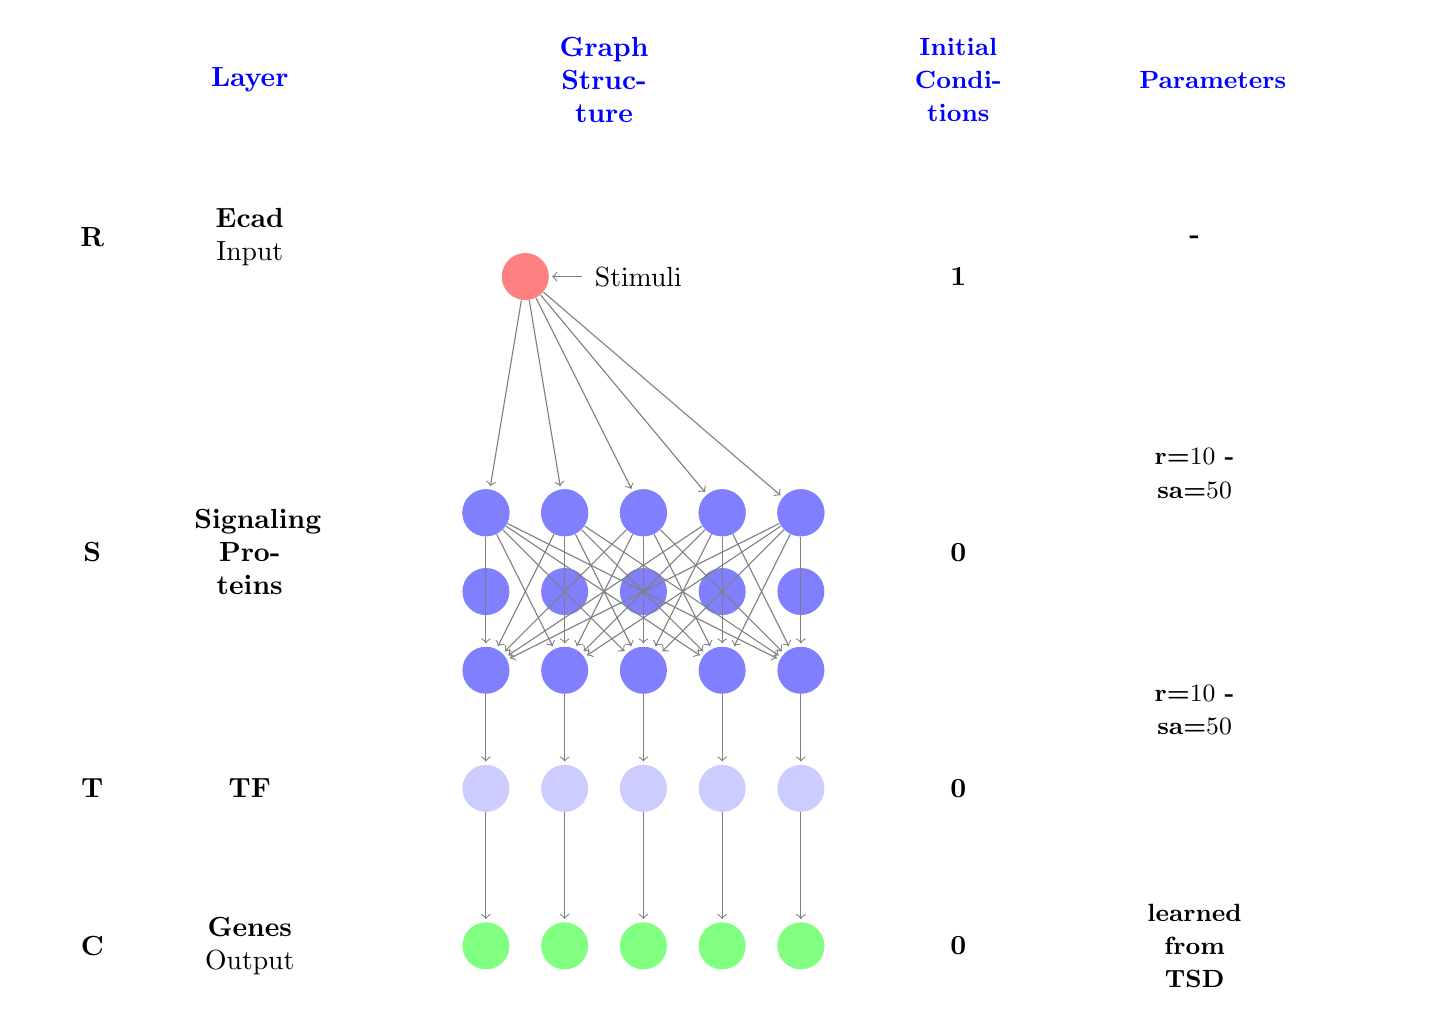
\begin{tikzpicture}[shorten >=1pt,->,draw=black!50, node distance=\layersep]
    \tikzstyle{every pin edge}=[<-,shorten <=1pt]
    \tikzstyle{neuron}=[circle,fill=black!25,minimum size=17pt,inner sep=0pt]
    \tikzstyle{input neuron}=[neuron, fill=green!50];
    \tikzstyle{output neuron}=[neuron, fill=red!50];
    \tikzstyle{hidden neuron}=[neuron, fill=blue!50];
    \tikzstyle{transfact neuron}=[neuron, fill=blue!20];
    \tikzstyle{annot} = [text width=4em, text centered]

    % Draw the input layer nodes
    \foreach \name / \x in {1,...,5}
    % This is the same as writing \foreach \name / \y in {1/1,2/2,3/3,4/4}
       % \node[input neuron, pin=left:Output \#\y] (I-\name) at (0,-\y) {};
         \node[input neuron] (I-\name) at (\x-7,-4) {};

     % Draw the transcription factor layer node
    \foreach \name / \x in {1,...,5}
    % This is the same as writing \foreach \name / \y in {1/1,2/2,3/3,4/4}
       % \node[input neuron, pin=left:Output \#\y] (I-\name) at (0,-\y) {};
         \node[transfact neuron] (TF-\name) at (\x-7,-2) {};
     
     
     % Draw the hidden layer nodes
    \foreach \name / \x in {1,...,5}
        \path[yshift=0.5cm]
           % node[hidden neuron] (H-\name) at (\layersep,-\y cm) {};
             node[hidden neuron] (H-\name) at (\x-7 , \layersep) {};
             
    
    % Draw the hidden layer nodes
    \foreach \name / \x in {1,...,5}
        \path[yshift=0.5cm]
           % node[hidden neuron] (H-\name) at (\layersep,-\y cm) {};
             node[hidden neuron] (H1-\name) at (\x-7 ,1) {};
             
     % Draw the hidden layer nodes 1
    \foreach \name / \x in {1,...,5}
        \path[yshift=0.5cm]
           % node[hidden neuron] (H-\name) at (\layersep,-\y cm) {};
             node[hidden neuron] (H2-\name) at (\x-7 ,0) {};
             
     % Draw the hidden layer nodes 2
    \foreach \name / \x in {1,...,5}
        \path[yshift=0.5cm]
           % node[hidden neuron] (H-\name) at (\layersep,-\y cm) {};
             node[hidden neuron] (H3-\name) at (\x-7 ,-1) {};
             
    % Draw the output layer node
     \node[output neuron,pin={[pin edge={<-}]right:Stimuli}] (O) at (2.5-8,4.5) {};
     
     
   %connect nodes   

    % Connect every node in the input layer with every node in the
    % hidden layer.
    \foreach \source in {1,...,5}
        \foreach \dest in {1,...,5}
            \path (H-\dest) edge (H3-\source);

    % Connect every node in the hidden layer with the output layer
    \foreach \source in {1,...,5}
        \path (O) edge (H-\source) ;
        
   %connect sp to tf
   \foreach \source in {1,...,5}
    \path (H3-\source) edge (TF-\source);
        
    %connect TF with Genes
    
    \foreach \source in {1,...,5}
     \path (TF-\source) edge (I-\source);
     
      %titre du graphe
    \node[annot] (graphTitle) at (2.5-7,7) {\textcolor{blue}{\textbf{Graph Structure}}};

    % Annotate the layers
    \node[annot] (layerTitle) at (-9,7) {\textcolor{blue}{\textbf{Layer}}};
    \node[annot, node distance=1cm] (couchesp) at (-9,1) {\textbf{Signaling Proteins} };
    \node[annot] (coucheFT) at (-9,-2) {\textbf{TF} };
    \node[annot] (coucheGene) at (-9,-4) {\textbf{Genes} Output };
    \node[annot] (noeudEntre) at (-9,5) {\textbf{Ecad} Input };
    
    %noeud pour ajouter le R S T C 
    \node[annot] (R) at (-11,5) {\textcolor{black}{\textbf{R}}};
    \node[annot] (S) at (-11,1) {\textcolor{black}{\textbf{S}}};
    \node[annot] (T) at (-11,-2) {\textcolor{black}{\textbf{T}}};
    \node[annot] (C) at (-11,-4) {\textcolor{black}{\textbf{C}}};
    \node[annot] (test) at (5,-4) {\textcolor{black}{\textbf{}}};
    
    %noeud pour les règles de modélisation
    \node[annot] (icTitle) at (0,7) {\textcolor{blue}{\textbf{\small Initial Conditions}}};
    \node[annot] (RMi) at (0,4.5) {\textcolor{black}{\textbf{1}}};
    \node[annot] (SMi) at (0,1) {\textcolor{black}{\textbf{0}}};
    \node[annot] (TMi) at (0,-2) {\textcolor{black}{\textbf{0}}};
    \node[annot] (CMi) at (0,-4) {\textcolor{black}{\textbf{0}}};
    %\node[annot] (P) at (5,-4) {\textcolor{black}{\huge \textbf{}}};
    
    %noeuds pour les hypothèses de modélisation
    \node[annot] (parameterTitle) at (3,7) {\textcolor{blue}{\small \textbf{Parameters}}};
    \node[annot] (RH) at (3,5) {\textcolor{black}{\textbf{-}}};
    \node[annot] (SH) at (3,2) {\textcolor{black}{\small \textbf{r=$10$ - sa=$50$}}};
    \node[annot] (TH) at (3,-1) {\textcolor{black}{\small \textbf{r=$10$ - sa=$50$}}};
    \node[annot] (CH) at (3,-4) {\textcolor{black}{\small \textbf{learned from TSD}}};
    %\node[annot] (test) at (5,-4) {\textcolor{black}{\huge \textbf{}}};
    
    %noeuds de repères pour les sous-graphs
    
    \node[annot] (R1) at (-4.7,\layersep) {};
    \node[annot] (R2) at (-4.7,1) {};
    \node[annot] (R3) at (-6.8,-1) {};
    \node[annot] (R4) at (-6.5,-4) {};
    \node[annot] (R5) at (-6.5,\layersep) {};
    
   
     
\end{tikzpicture}
}

 
 \caption{RSTC network structure and initial conditions assigned to each node in the layer}
 \label{fig:initialCondition}
\end{figure}

